%=====================================================================
%  HospitAI - Student conference presentation (CSSC)
%  Beamer, compile with pdflatex.  Author: Ioan-Iulian Todor
%
%  Build:  pdflatex HospitAI_presentation.tex   (twice, for the footline)
%  Figures are loaded from ./figs/
%=====================================================================
\documentclass[aspectratio=169,11pt]{beamer}

\usepackage[utf8]{inputenc}
\usepackage[T1]{fontenc}
\usepackage[english]{babel}
\usepackage{lmodern}
\usepackage{helvet}                 % modern sans-serif look
\renewcommand{\familydefault}{\sfdefault}
\usepackage{amsmath,amssymb}
\usepackage{booktabs}
\usepackage{array}
\usepackage{colortbl}   % \rowcolor in tables
\usepackage{tikz}
\usetikzlibrary{arrows.meta,positioning,shapes.geometric,calc,fit,backgrounds}

\graphicspath{{figs/}{./}}

%---------------------------------------------------------------------
%  COLOR PALETTE
%---------------------------------------------------------------------
\definecolor{hospblue}{HTML}{15324F}    % deep blue (primary)
\definecolor{hospblue2}{HTML}{1E4D74}   % medium blue
\definecolor{hospaccent}{HTML}{0E9594}  % medical teal (accent)
\definecolor{hospaccent2}{HTML}{27AE8F} % green
\definecolor{hosporange}{HTML}{E08A1E}  % orange (numeric highlight)
\definecolor{hosplight}{HTML}{EAF3F4}   % block background
\definecolor{hospgray}{HTML}{5B6B7B}    % secondary text
\definecolor{hosprule}{HTML}{0E9594}

%---------------------------------------------------------------------
%  THEME
%---------------------------------------------------------------------
\usetheme{default}
\usefonttheme{professionalfonts}
\setbeamertemplate{navigation symbols}{}

\setbeamercolor{normal text}{fg=hospblue!92!black,bg=white}
\setbeamercolor{structure}{fg=hospaccent}
\setbeamercolor{title}{fg=hospblue}
\setbeamercolor{frametitle}{fg=white,bg=hospblue}
\setbeamercolor{itemize item}{fg=hospaccent}
\setbeamercolor{itemize subitem}{fg=hospaccent2}
\setbeamercolor{enumerate item}{fg=hospaccent}
\setbeamercolor{block title}{bg=hospaccent,fg=white}
\setbeamercolor{block body}{bg=hosplight,fg=hospblue!92!black}
\setbeamercolor{block title alerted}{bg=hosporange,fg=white}
\setbeamercolor{block body alerted}{bg=hosporange!12,fg=hospblue!92!black}

\setbeamerfont{frametitle}{series=\bfseries,size=\large}
\setbeamerfont{title}{series=\bfseries}
\setbeamerfont{block title}{series=\bfseries,size=\small}

\setbeamertemplate{blocks}[rounded][shadow=false]
\setbeamertemplate{itemize item}{\small\raisebox{0.15ex}{\textbullet}}
\setbeamertemplate{itemize subitem}{\scriptsize\raisebox{0.15ex}{\textendash}}

%---------------------------------------------------------------------
%  Custom FRAMETITLE (band + accent line)
%---------------------------------------------------------------------
\setbeamertemplate{frametitle}{%
  \nointerlineskip
  \begin{beamercolorbox}[wd=\paperwidth,ht=2.7ex,dp=1.25ex,leftskip=0.55cm,rightskip=0.55cm]{frametitle}%
    \usebeamerfont{frametitle}\insertframetitle%
  \end{beamercolorbox}%
  \vskip-0.4pt%
  {\color{hosprule}\rule{\paperwidth}{2.2pt}}%
  \vskip0.35em
}

%---------------------------------------------------------------------
%  Custom FOOTLINE
%---------------------------------------------------------------------
\setbeamercolor{fl author}{bg=hospblue,fg=white}
\setbeamercolor{fl title}{bg=hospblue2,fg=white}
\setbeamercolor{fl num}{bg=hospaccent,fg=white}
\setbeamertemplate{footline}{%
  \leavevmode%
  \hbox{%
    \begin{beamercolorbox}[wd=.30\paperwidth,ht=2.6ex,dp=1.1ex,leftskip=.55cm]{fl author}%
      \usebeamerfont{author in head/foot}\footnotesize Ioan-Iulian Todor%
    \end{beamercolorbox}%
    \begin{beamercolorbox}[wd=.55\paperwidth,ht=2.6ex,dp=1.1ex,center]{fl title}%
      \usebeamerfont{title in head/foot}\footnotesize HospitAI - Patient Clustering, Sequence Mining \& AI Interpretation%
    \end{beamercolorbox}%
    \begin{beamercolorbox}[wd=.15\paperwidth,ht=2.6ex,dp=1.1ex,center]{fl num}%
      \usebeamerfont{title in head/foot}\footnotesize\insertframenumber\,/\,\inserttotalframenumber%
    \end{beamercolorbox}%
  }%
}

%---------------------------------------------------------------------
%  HELPER MACROS
%---------------------------------------------------------------------
% numeric highlight (key statistics)
\newcommand{\stat}[1]{{\color{hosporange}\bfseries #1}}
\newcommand{\kw}[1]{{\color{hospaccent}\bfseries #1}}

% formula box
\newcommand{\formulabox}[2]{%
  \begin{beamercolorbox}[wd=\linewidth,rounded=true,shadow=false,sep=6pt]{block body}%
    {\color{hospaccent}\footnotesize\bfseries #1}\\[2pt]%
    \centering #2%
  \end{beamercolorbox}}

% placeholder for images that do not exist yet (no tikz, robust)
\setlength{\fboxsep}{8pt}
\newcommand{\imgplaceholder}[3][0.9\linewidth]{%
  {\setlength{\fboxrule}{1pt}%
   \fcolorbox{hospaccent}{hosplight}{%
     \begin{minipage}[c][#2][c]{#1}
       \centering
       {\color{hospaccent}\bfseries\large [ IMAGE ]}\\[4pt]
       {\color{hospgray}\footnotesize #3}
     \end{minipage}}}}

% clinical arrow for sequences
\newcommand{\seqarrow}{\,{\color{hospaccent}\boldmath$\rightarrow$}\,}

%---------------------------------------------------------------------
%  SECTION DIVIDER
%---------------------------------------------------------------------
\AtBeginSection[]{%
  \begin{frame}[plain]
    \begin{tikzpicture}[remember picture,overlay]
      \fill[hospblue] (current page.south west) rectangle (current page.north east);
      \fill[hospaccent] ([yshift=-1.6cm]current page.west) rectangle ([yshift=-2.0cm]current page.east);
      \node[anchor=west,text=white] at ([xshift=1.2cm,yshift=1.1cm]current page.west)
        {\fontsize{56}{56}\selectfont\bfseries\color{hospaccent!85!white}\insertsectionnumber};
      \node[anchor=west,text=white,text width=0.8\paperwidth] at ([xshift=1.2cm,yshift=-0.7cm]current page.west)
        {\Huge\bfseries\insertsection};
    \end{tikzpicture}
  \end{frame}}

%=====================================================================
\begin{document}

%---------------------------------------------------------------------
%  SLIDE 1 - TITLE
%----------------------------------------------------
{\setbeamertemplate{footline}{}
\begin{frame}[plain]
  \begin{tikzpicture}[remember picture,overlay]
    % background
    \fill[hospblue] (current page.south west) rectangle (current page.north east);
    % bottom band
    \fill[hospblue2] (current page.south west) rectangle ([yshift=1.8cm]current page.south east);
    \draw[hospaccent,line width=2.5pt]
      ([yshift=1.8cm]current page.south west) -- ([yshift=1.8cm]current page.south east);

    % logo stanga in banda
    \node[anchor=west] at ([xshift=0.6cm,yshift=0.9cm]current page.south west)
      {
\includegraphics[height=1.3cm]{logo_utcn.png}};

    % text dreapta in banda
    \node[anchor=east, align=center] at ([xshift=-0.6cm,yshift=0.9cm]current page.south east){
      {\color{white}\footnotesize Technical University of Cluj-Napoca}\\
      {\color{white!75}\scriptsize Faculty of Automation and Computer Science}
    };

    % continut centrat vertical intre top si banda (banda incepe la 1.8cm, paperheight ~9.6cm)
    % centrul zonei utile = (paperheight - 1.8cm) / 2 + 1.8cm = ~5.7cm de la bottom
    \node[anchor=center, align=center, text width=0.85\paperwidth]
      at ([xshift=0cm,yshift=5.5cm]current page.south){
      {\color{white}\fontsize{40}{44}\selectfont\bfseries HospitAI}\\[8pt]
      {\color{hospaccent!80!white}\rule{4cm}{1pt}}\\[12pt]
      {\color{hosplight}\normalsize A hospital data analytics platform that combines}\\[3pt]
      {\color{hosplight}\normalsize patient grouping, clinical sequence mining,}\\[3pt]
      {\color{hosplight}\normalsize and AI-generated interpretation}\\[24pt]
      {\color{white}\large\bfseries Student: Ioan-Iulian Todor}\\[5pt]
      {\color{hospaccent!70!white}\small Advisors: Conf. Prof. Dr. Eng. Cristina Pop, Conf. Dr. Eng. Viorica Chifu}
    };
  \end{tikzpicture}
\end{frame}}

%---------------------------------------------------------------------
%  SLIDE 2 - OUTLINE
%---------------------------------------------------------------------
\begin{frame}{Outline}
  \vspace{0.5em}
  \begin{columns}[T]
    \begin{column}{0.48\textwidth}
      \begin{enumerate}
        \item[\textcolor{hospaccent}{\bfseries 1.}] Introduction and context
        \vspace{0.4em}
        \item[\textcolor{hospaccent}{\bfseries 2.}] Related work
        \vspace{0.4em}
        \item[\textcolor{hospaccent}{\bfseries 3.}] The HospitAI analytics pipeline\\
          {\footnotesize\color{hospgray} (methodology)}
        \vspace{0.4em}
        \item[\textcolor{hospaccent}{\bfseries 4.}] Simulations and experimental results
      \end{enumerate}
    \end{column}

    \begin{column}{0.48\textwidth}
      \begin{enumerate}
        \item[\textcolor{hospaccent}{\bfseries 5.}] Discussion and performance review
        \vspace{0.4em}
        \item[\textcolor{hospaccent}{\bfseries 6.}] Conclusions and future work
        \vspace{0.4em}
        \item[\textcolor{hospaccent}{\bfseries 7.}] References and math appendix
      \end{enumerate}
    \end{column}
  \end{columns}

  \vspace{0.35cm}

  \begin{block}{Overview}
    In short, \kw{HospitAI} is an \kw{end-to-end} analytics pipeline that ingests
    raw EHR data, applies \kw{unsupervised patient clustering} and
    \kw{clinical sequence mining}, and provides \kw{AI-generated}
    interpretations to support data-driven hospital insights.
  \end{block}
\end{frame}

%=====================================================================
\section{Introduction and context}
%=====================================================================

%---------------------------------------------------------------------
%  SLIDE 3 - Context and challenges
%---------------------------------------------------------------------
\begin{frame}{Context and challenges (EHR data)}
  \vspace{0.3em}
  \begin{itemize}\setlength{\itemsep}{0.6em}
    \item EHR (Electronic Health Record) systems gather huge volumes of clinical data, but most of it stays \kw{unused}. Also, querying it requires SQL expertise that most medical staff lack.
    \item A global analysis on that data hides \kw{patient diversity}: an acute case is very different from the many conditions of an elderly patient.
    \item Medical care is strongly \kw{time-based}. The order of actions matters more than how often they happen.
    \item Classic algorithms return lists of abstract codes that clinicians cannot interpret quickly.
  \end{itemize}
  \vfill
  {\color{hosprule}\rule{2.5pt}{1.1em}\hspace{6pt}%
   \kw{HospitAI} addresses these challenges with: patient grouping (clustering), clinical sequence mining, an AI interpretation layer, and an AI Chat Agent.}
\end{frame}
%---------------------------------------------------------------------
%  SLIDE 4 - Main objective and sub-objectives
%---------------------------------------------------------------------
\begin{frame}{Main objective and sub-objectives}
  \begin{block}{Main objective}
    \small Build the \kw{end-to-end} \textbf{HospitAI} pipeline that turns raw clinical data into explainable medical decisions.
  \end{block}
  \vspace{0.3em}
  \begin{block}{Sub-objectives}
    \small
    \begin{enumerate}\setlength{\itemsep}{0.25em}
      \item \kw{Patient grouping:} cluster patients into homogeneous groups using K-Prototypes on mixed-type data.
      \item \kw{Sequence mining:} extract and rank treatment patterns over time using PrefixSpan and GML score.
      \item \kw{AI verbalization:} generate readable clinical summaries per cluster via an LLM verbalizer.
      \item \kw{SQL agent:} allow patients or medical staff to query clinical data in plain English via a LangGraph agent; also responds to general health-related questions.
    \end{enumerate}
  \end{block}
\end{frame}

%=====================================================================
\section{Related work}
%=====================================================================

%---------------------------------------------------------------------
%  SLIDE 5 - Related work and gaps
%---------------------------------------------------------------------
\begin{frame}{Related work: what others did}
  \scriptsize
  \renewcommand{\arraystretch}{1.3}
  \begin{tabular}{@{}>{\raggedright}p{2.0cm} >{\raggedright}p{2.7cm} >{\raggedright\arraybackslash}p{7.3cm}@{}}
    \toprule
    \textbf{Category} & \textbf{Papers} & \textbf{What they do} \\
    \midrule
    Surveys &
      Rosa (2022), Flothow (2023) &
      Rosa distinguishes sequence mining from process mining in pathway analysis. Flothow separates full-trajectory clustering from subsequence pattern mining. \\
    Clustering and mining &
      Najjar (2018), Baudrier (2022), Vogt (2017) &
      Najjar clusters individual visits with K-Prototypes then derives pathways. Baudrier links trajectory clustering to outcomes in kidney cancer. Vogt clusters heart-failure pathways from insurance claims. \\
    Sequence mining &
      Perer (2015) &
      Mines frequent event sequences from EMRs and links them to patient outcomes via visual analytics. \\
    Patient clustering &
      Yang (2024), Aljohani (2024) &
      Yang clusters EHR patients to reveal health risks. Aljohani evaluates eight clustering methods for patient stratification. \\
    Process mining &
      Murazzano (2026) &
      Applies process mining to chronic respiratory patients, observing high variability in care processes. \\
    \bottomrule
  \end{tabular}
\end{frame}

%---------------------------------------------------------------------
%  SLIDE 5b - Related work: gaps and contribution
%---------------------------------------------------------------------
\begin{frame}{Related work: gaps and our contribution}
  \begin{columns}[T]
    \begin{column}{0.48\textwidth}
      \scriptsize
      \renewcommand{\arraystretch}{1.25}
      \begin{tabular}{@{}>{\raggedright}p{2.0cm} >{\raggedright\arraybackslash}p{3.6cm}@{}}
        \toprule
        \textbf{Category} & \textbf{Gap} \\
        \midrule
        Surveys & Overview only; no unified implementation \\[3pt]
        Clustering and mining & Visit-level grouping; single-disease scope; steps applied in a different order \\[3pt]
        Sequence mining & Frequency only; no clinical ranking metric to filter trivial patterns \\[3pt]
        Patient clustering & No sequential analysis component \\[3pt]
        Process mining & No AI interpretation or verbalization layer \\
        \bottomrule
      \end{tabular}
    \end{column}
    \begin{column}{0.52\textwidth}
      \begin{block}{What HospitAI adds}
        \scriptsize
        \begin{itemize}\setlength{\itemsep}{0.4em}
          \item \kw{Patient-level} mixed clustering with K-Prototypes across \stat{22,284} patients, not visit-level
          \item Cross-domain applicability, not limited to a single disease or patient type
          \item \kw{Clinically ranked} sequences via the GML score, which rewards genuine statistical association beyond raw frequency
          \item \kw{LLM verbalization} that generates readable cluster summaries for both clinicians and patients
          \item \kw{Natural-language SQL agent} built on LangGraph, enabling clinical queries without SQL expertise
        \end{itemize}
      \end{block}
    \end{column}
  \end{columns}
\end{frame}

%=====================================================================
\section{The HospitAI analytics pipeline}
%=====================================================================

%---------------------------------------------------------------------
%  SLIDE 6 - Architecture + ETL
%---------------------------------------------------------------------
\begin{frame}{Pipeline architecture and ETL (Stage 1)}
  \begin{columns}[T]
    \begin{column}{0.5\textwidth}
      \small
      \begin{itemize}
        \item The architecture is split in two: an offline analysis pipeline in \kw{Python} that processes raw EHR data and produces clustering and sequence mining results, and a fast web application (\kw{Next.js and FastAPI}) that displays those results and allows medical staff to perform CRUD operations on the data.
        \item \kw{Stage 1 - ETL (extract, transform and load):} Synthea complex synthetic EHR dataset (\stat{22,284} patients), used to ensure full \kw{privacy compliance} (GDPR). Missing values filled by \kw{mode / median}.
      \end{itemize}
    \end{column}
    \begin{column}{0.45\textwidth}
      \centering
      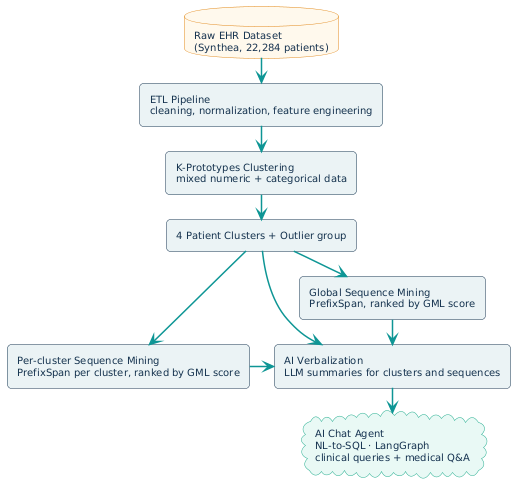
\includegraphics[width=\linewidth]{figure1.png}\\[2pt]
      {\scriptsize\color{hospgray} Fig.~1. The HospitAI pipeline}
    \end{column}
  \end{columns}
\end{frame}

%---------------------------------------------------------------------
%  SLIDE 7 - Clustering (K-Prototypes)
%---------------------------------------------------------------------
\begin{frame}{Patient Grouping (Stage 2)}
  \small
  \begin{itemize}\setlength{\itemsep}{0.5em}
    \item \kw{Why K-Prototypes:} it handles mixed data (numeric and categorical) natively. K-Means fails on categorical attributes; K-Modes fails on numeric ones.
    \item Many features were \kw{derived} from raw EHR data rather than read directly. For example, the \kw{clinical severity score} is computed from condition count, medication load, and procedure frequency.
    \item \kw{K=4} was selected via an \kw{elbow plot} on the Gower inertia curve, which showed a clear inflection point at 4 clusters.
    \item At cluster creation, the \kw{AI layer} receives the feature values via prompt and generates a \kw{title}, \kw{insights}, and \kw{recommendations} tailored to each patient group.
  \end{itemize}
  \begin{columns}[T]
    \begin{column}{0.6\textwidth}
      \formulabox{Huang mixed distance ($\gamma$ = categorical weight)}{%
        $\displaystyle d(X,Y)=\sum_{j=1}^{p}(x_j-y_j)^2+\gamma\!\!\sum_{j=p+1}^{m}\!\!\delta(x_j,y_j)$}
    \end{column}
    \begin{column}{0.4\textwidth}
      \formulabox{Outlier detection}{%
        $\displaystyle z=\frac{x-\mu}{\sigma}>6 \;\Rightarrow\; \text{class }(-1)$}
    \end{column}
  \end{columns}
\end{frame}

%---------------------------------------------------------------------
%  SLIDE 8 - Sequence mining
%---------------------------------------------------------------------
\begin{frame}{Sequence Mining (Stage 3)}
  \begin{columns}[T]
    \begin{column}{0.60\textwidth}
      \footnotesize
      \begin{itemize}\itemsep=2pt
        \item Patient timelines are built over a \kw{2-year window}; consecutive duplicates removed to avoid noise.
        \item \kw{PrefixSpan} extracts frequent subsequences with minimum support \stat{1\%}.
        \item \kw{Why not frequency alone:} common events carry no clinical signal. The \kw{GML score} measures genuine statistical association between events.
        \item A \kw{diversity bonus} rewards patterns mixing medications, procedures, and observations.
        \item Mining runs at \kw{two levels}: globally and per cluster.
      \end{itemize}
      \vspace{0.2em}
      \formulabox{GML score}{%
        $\displaystyle \mathrm{GML}(p)=\frac{s(p)/n}{\left(\prod_{i\in p}s(i)/n\right)^{1/k}}$}
    \end{column}
    \begin{column}{0.45\textwidth}
      \centering
      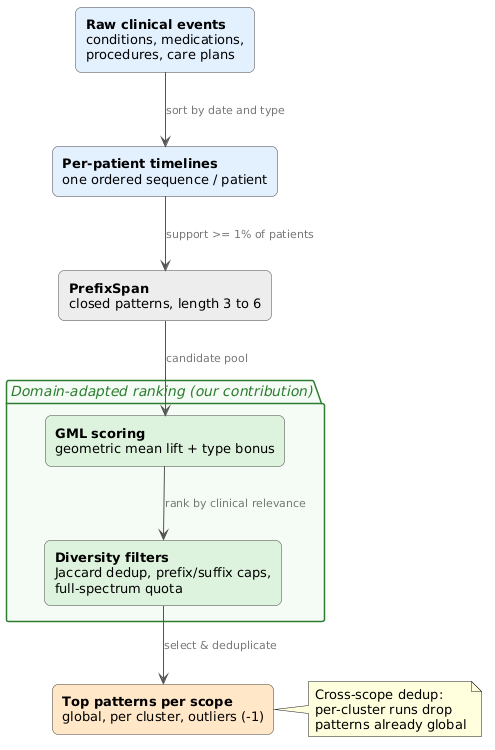
\includegraphics[height=0.72\textheight]{sequence_mining_pipeline.png}\\[1pt]
      {\scriptsize\color{hospgray} Fig.~2. The sequence mining pipeline}
    \end{column}
  \end{columns}
\end{frame}
%---------------------------------------------------------------------
%  SLIDE 9 - AI layer + SQL agent
%---------------------------------------------------------------------
\begin{frame}{The AI layer and the SQL agent (Stage 4)}
  \begin{columns}[T]
    \begin{column}{0.60\textwidth}
      \footnotesize
      \textbf{AI Verbalization}
      \begin{itemize}\setlength{\itemsep}{0.25em}
        \item Clusters are interpreted \kw{automatically at creation}: the LLM generates a \kw{title}, \kw{description}, \kw{insights}, and \kw{recommendations} from precomputed feature values.
        \item Interpretation can also be \kw{triggered on demand}.
        \item Two output modes: \kw{medical-oriented} (clinicians) and \kw{patient-oriented} (plain language).
        \item \kw{Sequences} can also be verbalized by the AI layer.
      \end{itemize}
      \vspace{0.4em}
      \textbf{SQL Agent}
      \begin{itemize}\setlength{\itemsep}{0.25em}
        \item Translates natural language to SQL; behavior adapts to \kw{user role}.
        \item Answers general medical questions with a disclaimer: responses are \kw{not a substitute for a doctor}.
        \item Out-of-scope questions are \kw{refused}.
      \end{itemize}
    \end{column}
    \begin{column}{0.48\textwidth}
      \centering
      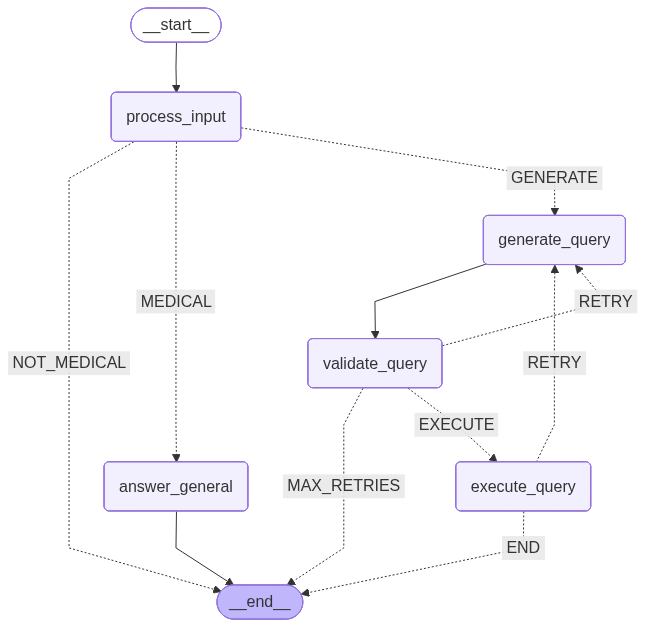
\includegraphics[width=0.92\linewidth]{high_level_architecture.png}\\
      {\scriptsize\color{hospgray} Fig.~3. The agent state machine (LangGraph)}
    \end{column}
  \end{columns}
\end{frame}

%=====================================================================
\section{Simulations and experimental results}
%=====================================================================

%---------------------------------------------------------------------
%  SLIDE 10 - Experimental setup
%---------------------------------------------------------------------
\begin{frame}{Simulation: experimental setup and data}
  \small
  \begin{itemize}
    \item After ETL, in Stage 2, most features that will be used for clustering are extracted through \kw{SQL aggregation queries} over the raw EHR tables.
    \item Some are \kw{derived} from others via feature engineering, e.g., tabulating clinical events into scores or ratios. Below there are listed all the features.
  \end{itemize}
  \vspace{0.2em}
  \centering
  \tiny
  \renewcommand{\arraystretch}{1.15}
  \begin{tabular}{@{}>{\raggedright\arraybackslash}p{2.0cm} >{\raggedright\arraybackslash}p{9.8cm}@{}}
    \toprule
    \textbf{Group} & \textbf{Features} \\
    \midrule
    Demographics &
      age, gender, race, ethnicity, marital status \\
    Encounter utilization &
      inpatient, outpatient, emergency, wellness, ambulatory, urgentcare, SNF, hospice counts;
      dominant encounter class; total encounter duration (hours); days since last encounter;
      routine care count, acute care count, severe care count \textit{(derived)};
      preventive-to-reactive ratio \textit{(derived)}; out-of-hours flyer; has inpatient history; readmission risk tier \\
    Conditions &
      total conditions, active conditions count, condition burden \textit{(derived: low/medium/high)};
      has\_diabetes, has\_hypertension, has\_heart\_disease, has\_cancer, has\_kidney\_disease,
      has\_mental\_health, respiratory disease profile \\
    Medications and procedures &
      total medications, lifetime medication days, is\_polypharmacy, medication intensity \textit{(derived: low/medium/high)},
      pain management tier; total procedures;
      clinical severity score \textit{(PCA-derived from procedures, medications, and active conditions)} \\
    Vitals and observations &
      avg BMI, BMI type \textit{(derived: Underweight to Obese III)};
      avg systolic BP, BP risk category \textit{(derived)};
      avg glucose, glucose risk category \textit{(derived: Normal/Prediabetic/Diabetic)};
      QALY, DALY \\
    Behavioral and risk &
      substance use profile, smoking status, cholesterol risk category,
      pregnancy history; distinct providers seen; dominant care plan \\
    \bottomrule
  \end{tabular}
\end{frame}


%---------------------------------------------------------------------
%  SLIDE 11 - Cluster descriptions and quality
%---------------------------------------------------------------------
\begin{frame}{Results: the obtained clusters}
  \begin{columns}[T]
    \begin{column}{0.56\textwidth}
      \small
      \begin{itemize}\setlength{\itemsep}{0.01em}
        \item \kw{Cluster 0 (Young Injury):} young patients, acute trauma, emergency and urgentcare encounters, low chronic burden.
        \item \kw{Cluster 1 (Maternity):} predominantly female, maternal care plans, low medication load, wellness encounters.
        \item \kw{Cluster 2 (Older High Risk):} elderly, polypharmacy, hypertension, diabetes, heart disease, long encounter duration.
        \item \kw{Cluster 3 (Pediatrics):} children, minimal active conditions, low procedure counts, wellness dominant.
        \item \kw{Cluster ($-1$) (Outliers):} extreme cases (oncology, dialysis, terminal care), stored separately for independent analysis.
      \end{itemize}
    \end{column}
    \begin{column}{0.44\textwidth}
      \begin{block}{Why the clusters are good}
        \small
        \begin{itemize}\setlength{\itemsep}{0.4em}
          \item Each cluster maps to a \kw{recognizable patient type} that a clinician can immediately interpret.
          \item The separation is driven by \kw{clinical behavior}: conditions, medications, and encounter patterns, not superficial demographics.
          \item Each group has a \kw{distinct care trajectory} that justifies different treatment and prevention strategies.
        \end{itemize}
      \end{block}
    \end{column}
  \end{columns}
\end{frame}

%---------------------------------------------------------------------
%  SLIDE 11c - Cluster heatmap
%---------------------------------------------------------------------
\begin{frame}{Results: cluster profiles}
  \centering
  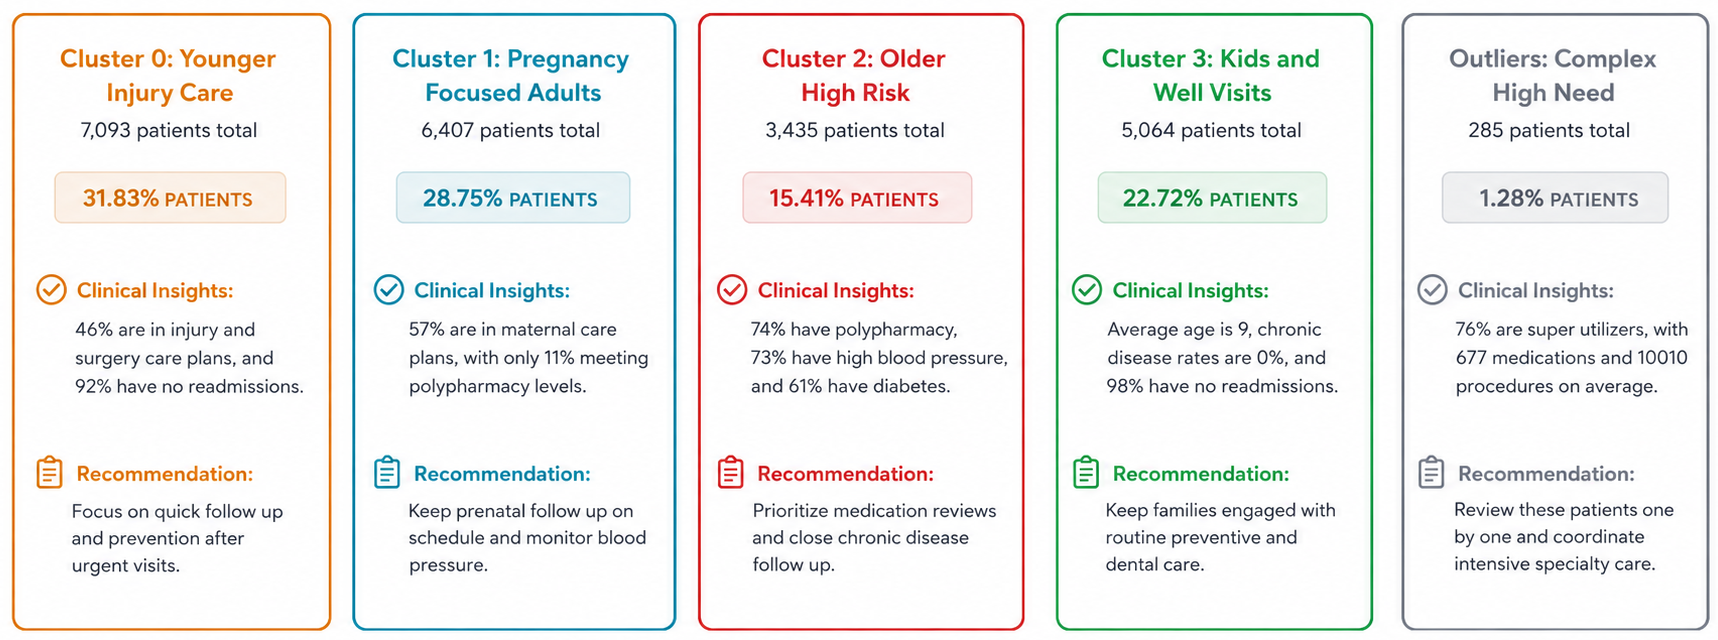
\includegraphics[height=0.60\textheight]{cluster_heatmap.png}\\[2pt]
  {\scriptsize\color{hospgray} Fig.~4. The obtained cluster profiles - fully AI interpreted}
\end{frame}

%---------------------------------------------------------------------
%  SLIDE 11d - Meaningful sequences
%---------------------------------------------------------------------
\begin{frame}{Results: meaningful clinical sequences (length 4--5)}
  \vspace{-0.15em}
  {\small PrefixSpan (min.\ support 1\%), sequences of length 4--5 ranked by \kw{GML score}. Top non-dental patterns per cluster:}
  \vspace{0.2em}
  \centering
  \tiny
  \renewcommand{\arraystretch}{1.22}
  \begin{tabular}{@{}>{\bfseries}p{2.4cm} >{\raggedright\arraybackslash}p{9.2cm} c@{}}
    \toprule
    \rowcolor{hosplight}
    C0 (Young Injury) & Laceration \seqarrow Wound care \seqarrow Suture open wound \seqarrow Acetaminophen & 0.30 \\
    \rowcolor{hosplight}
    C0 (Young Injury) & Acute bronchitis \seqarrow Respiratory therapy \seqarrow Resp.\ measurement \seqarrow Acetaminophen & 0.44 \\
    \midrule
    C1 (Maternity) & Tubal ligation (history) \seqarrow Minor surgery care \seqarrow Bilateral tubal ligation \seqarrow Postoperative care & 0.81 \\
    C1 (Maternity) & Miscarriage \seqarrow Normal pregnancy \seqarrow Standard pregnancy test \seqarrow Fetal ultrasound & 0.37 \\
    \midrule
    \rowcolor{hosplight}
    C2 (Older High Risk) & Fluticasone/Salmeterol inhaler \seqarrow Albuterol \seqarrow Pulmonary rehabilitation \seqarrow Spirometry & 0.70 \\
    \rowcolor{hosplight}
    C2 (Older High Risk) & Oxygen administration \seqarrow Prone positioning \seqarrow Furosemide inj.\ \seqarrow Heart failure education & 0.61 \\
    \midrule
    C3 (Pediatrics) & Fracture of bone \seqarrow Fracture of clavicle \seqarrow Orthopedic admission \seqarrow Clavicle X-ray & 0.62 \\
    C3 (Pediatrics) & Fracture of ankle \seqarrow Fracture of bone \seqarrow Fracture care \seqarrow Bone immobilization \seqarrow Ankle X-ray & 0.44 \\
    \midrule
    \rowcolor{hosplight}
    C($-1$) (Outliers) & Renal dialysis \seqarrow Epoetin Alfa \seqarrow Renal dialysis \seqarrow Epoetin Alfa & 0.77 \\
    \rowcolor{hosplight}
    C($-1$) (Outliers) & Chemo+radiation \seqarrow Cisplatin \seqarrow Paclitaxel \seqarrow Chemo+radiation \seqarrow Hospice care & 0.72 \\
    \bottomrule
  \end{tabular}\\[4pt]
  {\scriptsize\color{hospgray} Table 1: Suggestive sequences of length 4--5 per cluster (GML score)}
\end{frame}

%---------------------------------------------------------------------
%  SLIDE 12 - Dashboard + SQL agent validation
%---------------------------------------------------------------------
\begin{frame}{Results: cluster interpretation and Chat Agent}
  \begin{columns}[T]
    \begin{column}{0.50\textwidth}
      \centering
      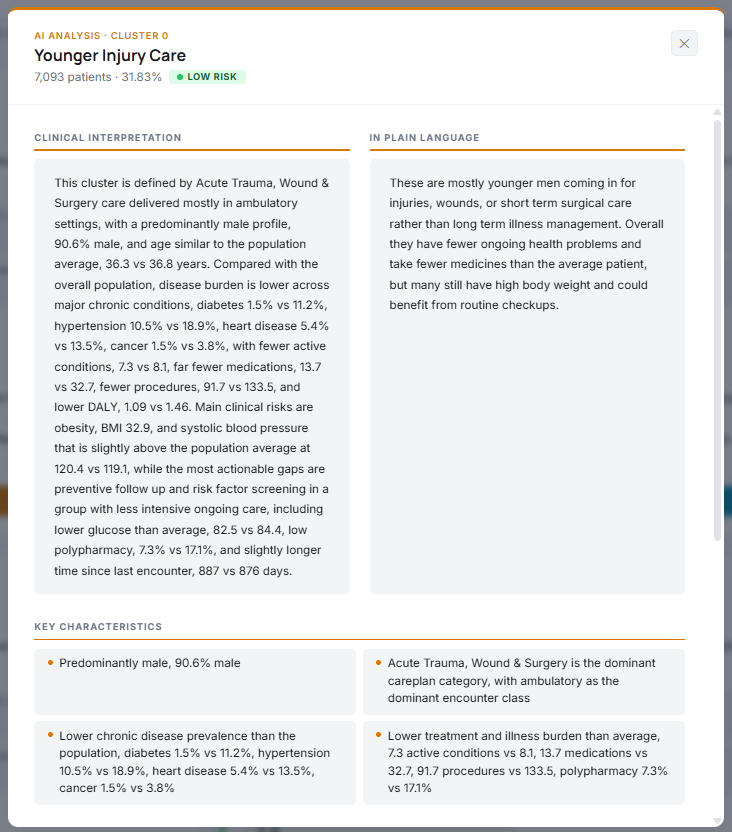
\includegraphics[width=\linewidth,height=0.72\textheight,keepaspectratio]{platform_interpretation.png}\\[3pt]
      {\scriptsize\color{hospgray} Fig.~5. AI-generated cluster interpretation}
    \end{column}
    \begin{column}{0.50\textwidth}
      \centering
      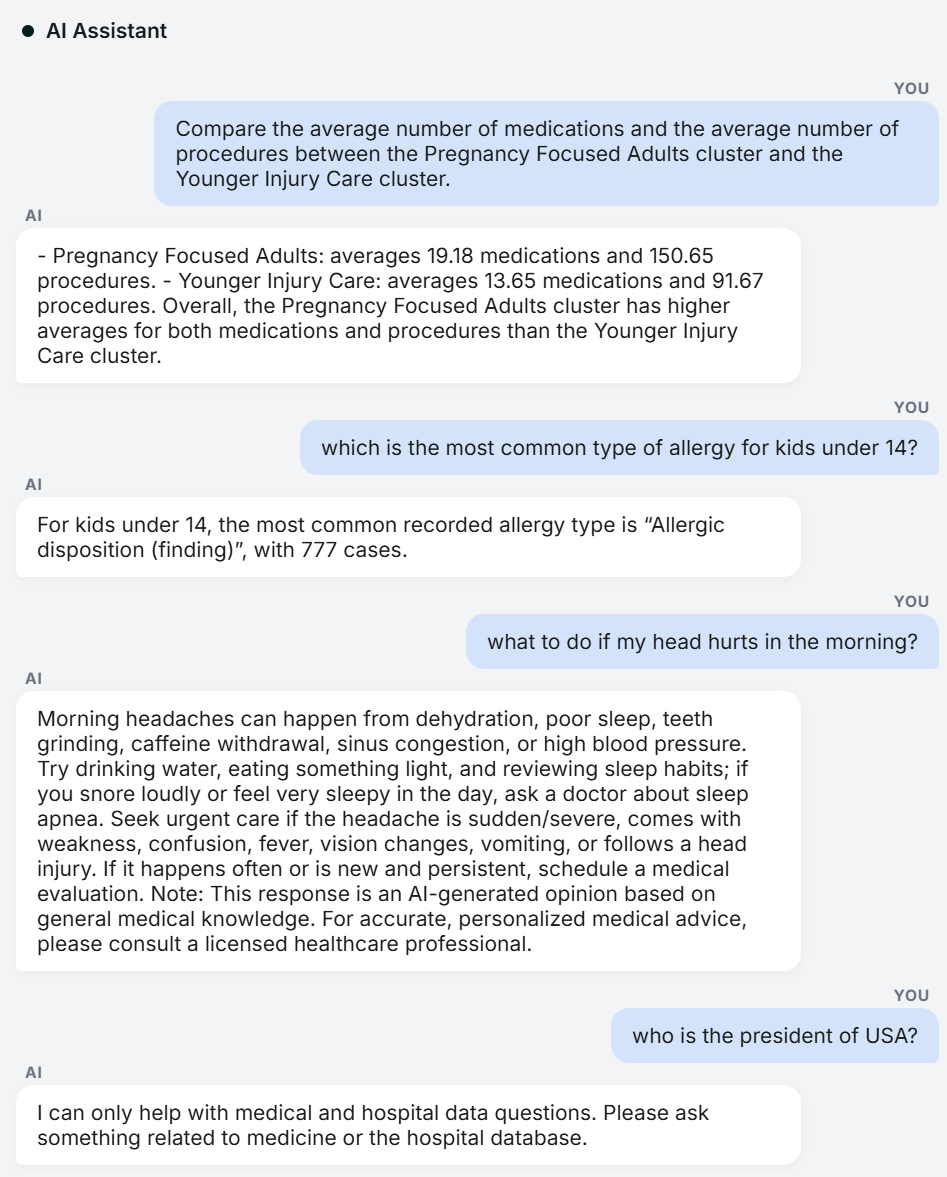
\includegraphics[width=\linewidth,height=0.72\textheight,keepaspectratio]{chatbot.png}\\[3pt]
      {\scriptsize\color{hospgray} Fig.~6. Chat Agent - example interaction}
    \end{column}
  \end{columns}
\end{frame}

%=====================================================================
\section{Discussion and performance review}
%=====================================================================

%---------------------------------------------------------------------
%  SLIDE 13 - Hyperparameter tuning
%---------------------------------------------------------------------
\begin{frame}{Discussion: benchmark logic and results validation}
  \begin{columns}[T]
    \begin{column}{0.65\textwidth}
      \scriptsize
      \begin{itemize}\setlength{\itemsep}{0.3em}
        \item \stat{629} total runs across \stat{60} feature configurations (v1--v60). Each config defines a distinct set of numerical and categorical features.
        \item Per config, a \kw{nested loop} varied: $k \in \{3,4,5,6\}$ and Z-score threshold $\in \{4,6\}$. For the best candidates, gamma $\in \{\text{auto},\,0.07,\,0.13,\,0.17\}$ and random seed $\in \{7,\,42,\,100\}$ were also tested.
        \item Each run was evaluated with three metrics: \kw{Gower Silhouette}, \kw{Calinski--Harabasz}, and \kw{Davies--Bouldin}, combined via a min-max normalized empirical score. Runs that split patients only by gender were excluded.
        \item Runs were sorted by score; the best configuration per $k \in \{4,5,6\}$ was selected (see table).
        \item For \kw{sequence mining}: patterns ranked by \kw{GML} (geometric mean lift). A \kw{diversity bonus} $(1+0.3\,(t-1))$ rewards patterns spanning multiple event types.
      \end{itemize}
      \vspace{0.25em}
      \formulabox{Optimization score (min-max normalized, empiric)}{%
        $\text{Score}=0.5\,\text{Gower}+0.3\,CH_{n}+0.2\,DB_{\mathit{inv}}$}
    \end{column}
    \begin{column}{0.35\textwidth}
      \centering
      \scriptsize
      \renewcommand{\arraystretch}{1.2}
      \begin{tabular}{@{}l c c c@{}}
        \toprule
        Config & $k$ & Gower & Score \\
        \midrule
        \rowcolor{hosplight}\textbf{v55} & \textbf{4} & \textbf{0.350} & \textbf{0.82} \\
        v40 & 5 & 0.324 & 0.74 \\
        v60 & 6 & 0.287 & 0.70 \\
        \bottomrule
      \end{tabular}

      \renewcommand{\arraystretch}{1.2}
      \begin{tabular}{@{}>{\bfseries}p{1.7cm} >{\raggedright\arraybackslash}p{4.1cm}@{}}
        \toprule
        \multicolumn{2}{@{}l@{}}{\color{hospaccent}\bfseries v55 feature set ($k=4$)} \\
        \midrule
        Numerical (5) & age, active conditions, total medications, total procedures, prev./reactive ratio \\[3pt]
        Categorical (8) & gender, pregnancy history, heart disease, diabetes, hypertension, condition burden, BMI type, dominant care plan \\
        \bottomrule
      \end{tabular}\\[4pt]
      {\scriptsize\color{hospgray} Table~2: v55 feature set. Results above are based on these features.}
    \end{column}
  \end{columns}
\end{frame}

%=====================================================================
\section{Conclusions and future work}
%=====================================================================

%---------------------------------------------------------------------
%  SLIDE 14 - Conclusions
%---------------------------------------------------------------------
\begin{frame}{Conclusions and future work}
  \begin{block}{Contribution}
    HospitAI shows that \kw{joining} mixed clustering with ranked mining turns the noise in EHR data into \kw{clear medical paths}.
  \end{block}
  \vspace{0.18em}
  \begin{block}{What the results enable}
    \small
    \begin{itemize}\setlength{\itemsep}{0.2em}
      \item \kw{Clusters} support risk stratification and targeted resource allocation per patient group.
      \item \kw{Sequences} can seed or validate clinical treatment protocols and guidelines.
    \end{itemize}
  \end{block}
  \vspace{0.15em}
  \begin{columns}[T]
    \begin{column}{0.5\textwidth}
      \small\textbf{Limitations}
      \begin{itemize}
        \item \kw{Synthetic} data (Synthea).
        \item It relies on an external language model, which raises hospital governance concerns.
      \end{itemize}
    \end{column}
    \begin{column}{0.5\textwidth}
      \small\textbf{Future work}
      \begin{itemize}
        \item Direct clinical review with specialist doctors.
        \item Testing on \kw{real}, anonymized databases.
      \end{itemize}
    \end{column}
  \end{columns}
\end{frame}

%---------------------------------------------------------------------
%  SLIDE 15 - References
%---------------------------------------------------------------------
\begin{frame}{References}
  \scriptsize
  \begin{columns}[T]
    \begin{column}{0.5\textwidth}
      \begin{itemize}\setlength{\itemsep}{0.3em}
        \item Z. Huang (1998). \textit{Extensions to the k-Means Algorithm for Clustering Large Data Sets with Categorical Values.} Data Mining and Knowledge Discovery.
        \item J. Pei et al. (2004). \textit{Mining Sequential Patterns by Pattern-Growth: The PrefixSpan Approach.} IEEE TKDE.
        \item A. Perer et al. (2015). \textit{Mining and exploring care pathways from EMR with visual analytics.} J. of Biomedical Informatics.
        \item A. Najjar et al. (2018). \textit{A two-step approach for mining patient treatment pathways.} Artificial Intelligence in Medicine.
        \item V. Vogt et al. (2018). \textit{Applying sequence clustering techniques to explore ambulatory care pathways.} European Journal of Public Health.
        \item C. Rosa et al. (2022). \textit{Modelling and Mining of Patient Pathways: A Scoping Review.} arXiv.
      \end{itemize}
    \end{column}
    \begin{column}{0.5\textwidth}
      \begin{itemize}\setlength{\itemsep}{0.3em}
        \item C. Baudrier et al. (2022). \textit{Combining sequence pattern mining with care trajectory clustering in kidney cancer patients.} Health Informatics Journal.
        \item A. Flothow et al. (2023). \textit{Analytical methods for identifying sequences of utilization in health data.} BMC Med. Research Methodology.
        \item W.-C. Yang et al. (2024). \textit{Using Medical Data and Clustering Techniques for a Smart Healthcare System.} Electronics.
        \item A. Aljohani (2024). \textit{Optimizing Patient Stratification in Healthcare: A Comparative Analysis of Clustering Algorithms for EHR Data.} Int. J. Computational Intelligence Systems.
        \item L. Murazzano et al. (2026). \textit{Clinical pathways discovery for long-term and chronic patients: A process mining approach.} Computers in Biology and Medicine.
      \end{itemize}
    \end{column}
  \end{columns}
\end{frame}

%---------------------------------------------------------------------
%  SLIDE 16 - Q&A
%---------------------------------------------------------------------
{\setbeamertemplate{footline}{}
\begin{frame}[plain]
  \begin{tikzpicture}[remember picture,overlay]
    \fill[hospblue] (current page.south west) rectangle (current page.north east);
  \end{tikzpicture}
  \begin{center}
    \vspace*{\fill}
    {\color{white}\fontsize{40}{44}\selectfont\bfseries Q\,\&\,A}\\[20pt]
    {\color{hosplight}\Large Thank you for your attention!}
    \vspace*{\fill}
  \end{center}
\end{frame}}

%=====================================================================
%  APPENDIX - BACKUP SLIDES (formulas)
%=====================================================================
\appendix
\section{Appendix: formulas}

%---------------------------------------------------------------------
%  SLIDE 17 - Formulas I
%---------------------------------------------------------------------
\begin{frame}{Appendix I: clustering and ETL pipeline}
  \small
  \begin{block}{K-Prototypes distance (Huang)}
    \centering
    $\displaystyle d(X,Y)=\sum_{j=1}^{p}(x_j-y_j)^2+\gamma\sum_{j=p+1}^{m}\delta(x_j,y_j),\qquad
      \delta(x_j,y_j)=\begin{cases}0,&x_j=y_j\\[2pt]1,&x_j\neq y_j\end{cases}$
  \end{block}
  \begin{columns}[T]
    \begin{column}{0.5\textwidth}
      \begin{block}{Outlier detection (Z-score, post-log)}
        \centering
        $\displaystyle z=\frac{x-\mu}{\sigma}\;\Rightarrow\; z>6 \Rightarrow \text{class }(-1)$
      \end{block}
    \end{column}
    \begin{column}{0.5\textwidth}
      \begin{block}{Scaling and normalization}
        \centering
        $\displaystyle X_{norm}=\frac{\ln(X)-\min(\ln X)}{\max(\ln X)-\min(\ln X)}$
      \end{block}
    \end{column}
  \end{columns}
\end{frame}

%---------------------------------------------------------------------
%  SLIDE 18 - Formulas II
%---------------------------------------------------------------------
\begin{frame}{Appendix II: sequence mining and evaluation}
  \small
  \begin{block}{Geometric Mean Lift (GML), base form}
    \centering
    $\displaystyle \mathrm{GML}(p)=\frac{s(p)/n}{\left(\prod_{i\in p}s(i)/n\right)^{1/k}}$
  \end{block}
  \begin{block}{Final GML (with a diversity bonus, $t$ = number of event types)}
    \centering
    $\displaystyle \mathrm{GML}_{final}(p)=\mathrm{GML}(p)\cdot\bigl(1+0.3\,(t-1)\bigr)$
  \end{block}
  \begin{block}{Weighted linear optimization (hyperparameter tuning)}
    \centering
    $\displaystyle \text{Score}_{config}=0.5\cdot\text{Gower}_{norm}+0.3\cdot CH_{norm}+0.2\cdot DB_{inv\_norm}$
  \end{block}
\end{frame}

\end{document}
